\question{Двойной интеграл. Определение и свойства.}

\setlength{\columnseprule}{1pt}
\begin{multicols}{2}
\begin{figure}[H]
  \centering

  \begin{subfigure}[b]{0.2\textwidth}
    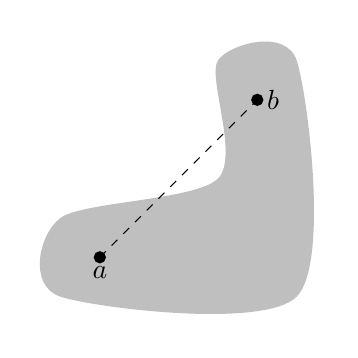
\begin{tikzpicture}

      \fill[lightgray] plot [smooth cycle] coordinates {
        (0, 0) (0, 1) (2, 1.5) (2, 3) (3, 3) (3, 0)
      };
      \draw[dashed] (0.5, 0.5) -- (2.5, 2.5);
      \draw[fill = black] (0.5, 0.5) circle (2pt) node[below] {\(a\)};
      \draw[fill = black] (2.5, 2.5) circle (2pt) node[right] {\(b\)};

    \end{tikzpicture}
  \caption{Невыпуклая область}\label{fig:area-prop-1-a}
  \end{subfigure}
  \qquad
  \begin{subfigure}[b]{0.2\textwidth}
    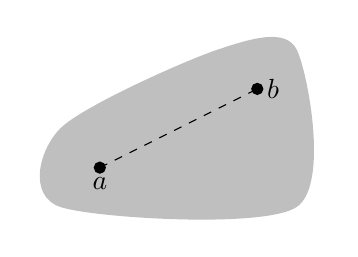
\begin{tikzpicture}

      \fill [lightgray] plot [smooth cycle] coordinates {
        (0, 0) (0, 1)  (2, 2) (3, 2) (3, 0)
      };
      \draw[dashed] (0.5, 0.5) -- (2.5, 1.5);
      \draw[fill = black] (0.5, 0.5) circle (2pt) node[below] {\(a\)};
      \draw[fill = black] (2.5, 1.5) circle (2pt) node[right] {\(b\)};

    \end{tikzpicture}
    \caption{Выпуклая область}\label{fig:area-prop-1-b}
  \end{subfigure}
\end{figure}

\begin{figure}[H]
  \centering

  \begin{subfigure}[b]{0.2\textwidth}
    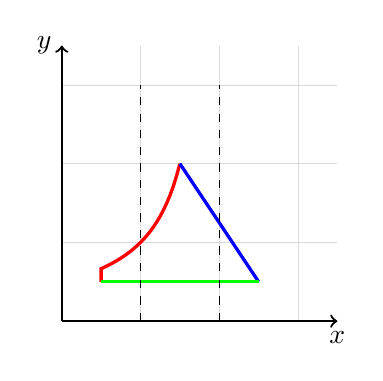
\begin{tikzpicture}

      \draw[very thin, gray!30, step = 1cm] (0, 0) grid (3.5, 3.5);
      \draw[color = red, very thick, domain = 0.5 : 1.5, variable = \x]
        (0.5, 0.5)
        -- plot ({\x}, {-1 / (\x - 2)});
      \draw[color = blue, very thick, domain = 1.5 : 2.5, variable = \x]
        (1.5, 2)
        -- plot ({\x}, {-1.5 * \x + 4.25});
      \draw[color = green, very thick] (0.5, 0.5) -- (2.5, 0.5);
    
      \draw[thick] [->] (0, 0) -- (3.5, 0) node[right, below] {\(x\)};
      \draw[thick] [->] (0, 0) -- (0, 3.5) node[above, left] {\(y\)};
      \draw[dashed] (1, 0) -- (1, 3);
      \draw[dashed] (2, 0) -- (2, 3);

    \end{tikzpicture}
  \caption{Неправильная в направлении \(Oy\) область}\label{fig:area-prop-2-a}
  \end{subfigure}
  \qquad
  \begin{subfigure}[b]{0.2\textwidth}
    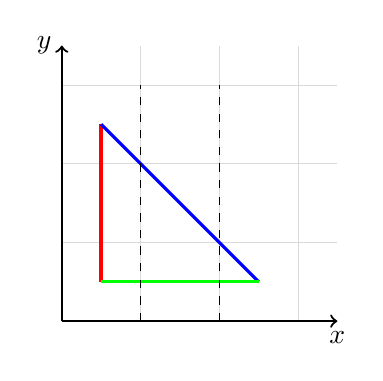
\begin{tikzpicture}

      \draw[very thin, gray!30, step = 1cm] (0, 0) grid (3.5, 3.5);
      \draw[color = red, very thick] (0.5, 0.5) -- (0.5, 2.5);
      \draw[color = blue, very thick] (0.5, 2.5) -- (2.5, 0.5);
      \draw[color = green, very thick] (0.5, 0.5) -- (2.5, 0.5);
    
      \draw[thick] [->] (0, 0) -- (3.5, 0) node[right, below] {\(x\)};
      \draw[thick] [->] (0, 0) -- (0, 3.5) node[above, left] {\(y\)};
      \draw[dashed] (1, 0) -- (1, 3);
      \draw[dashed] (2, 0) -- (2, 3);

    \end{tikzpicture}
    \caption{Правильная в направлении \(Oy\) область}\label{fig:area-prop-2-b}
  \end{subfigure}
\end{figure}

\columnbreak

\begin{figure}[H]
  \centering

  \begin{subfigure}[b]{0.2\textwidth}
    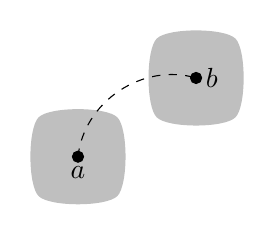
\begin{tikzpicture}
      \fill [lightgray] plot [smooth cycle] coordinates {
        (0, 0) (0, 1)  (1, 1) (1, 0)
      };
      \fill [lightgray] plot [smooth cycle] coordinates {
        (2.5, 1) (2.5, 2)  (1.5, 2) (1.5, 1)
      };
      \draw[dashed] (0.5, 0.5) edge[bend left = 50] (2, 1.5);
      \draw[fill = black] (0.5, 0.5) circle (2pt) node[below] {\(a\)};
      \draw[fill = black] (2, 1.5) circle (2pt) node[right] {\(b\)};
    \end{tikzpicture}

  \caption{Несвязная область}\label{fig:area-prop-3-a}
  \end{subfigure}
  \qquad
  \begin{subfigure}[b]{0.2\textwidth}
    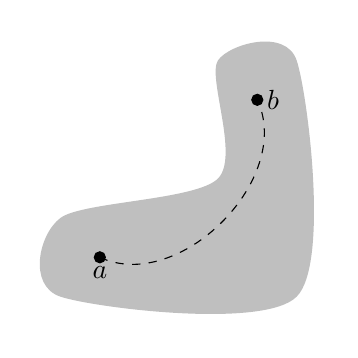
\begin{tikzpicture}

      \fill [lightgray] plot [smooth cycle] coordinates {
        (0, 0) (0, 1) (2, 1.5) (2, 3) (3, 3) (3, 0)
      };
      \draw[dashed] (0.5, 0.5) edge[bend right = 70] (2.5, 2.5);
      \draw[fill = black] (0.5, 0.5) circle (2pt) node[below] {\(a\)};
      \draw[fill = black] (2.5, 2.5) circle (2pt) node[right] {\(b\)};

    \end{tikzpicture}
    \caption{Связная область}\label{fig:area-prop-3-b}
  \end{subfigure}
\end{figure}

\begin{figure}[H]
  \centering

  \begin{subfigure}[b]{0.2\textwidth}
    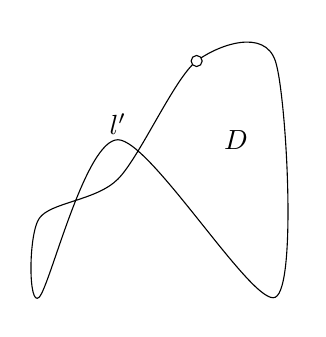
\begin{tikzpicture}
      
      \draw plot [smooth cycle] coordinates {
        (0, 0) (0, 1) (1, 1.5) (2, 3) (3, 3) (3, 0) (1, 2)
      };
      \draw[draw = black, fill = white] (2, 3) circle (2pt);
      \draw node at (2.5, 2) {\(D\)};
      \draw node at (1, 2.2) {\(l'\)};

    \end{tikzpicture}

  \caption{\(l'\) - не простая граница}\label{fig:area-prop-4-a}
  \end{subfigure}
  \qquad
  \begin{subfigure}[b]{0.2\textwidth}
    \begin{tikzpicture}

      \draw plot [smooth cycle] coordinates {
        (0, 0) (0, 1) (1, 1.5) (2, 3) (3, 3) (3, 0)
      };
      \draw node at (2, 1) {\(D\)};
      \draw node at (1, 2) {\(l\)};

    \end{tikzpicture}
    \caption{\(l\) - простая граница}\label{fig:area-prop-4-b}
  \end{subfigure}
\end{figure}
\end{multicols}
\setlength{\columnseprule}{0pt}

\begin{remark}
  Об области \(D\)

  Область \(D\) должна быть:
  \begin{enumerate}
    \item Выпуклой (\ref{fig:area-prop-1-b}), т.е. любые две точки можно стянуть
    отрезком, который полностью содержится в области \(D\).

    \item Правильной в координатном направлений. На рисунке
    \ref{fig:area-prop-2-a} отрезки, параллельные \(Oy\), при 'выходе' из
    области пересекают красную и синюю границы, которые имеют разное
    аналитическое задание. В то время как на рисунке \ref{fig:area-prop-2-b}
    отрезки 'входят' в область через зеленую границу, а 'выходят'
    \textbf{только} через синюю.

    \item Связной (\ref{fig:area-prop-3-b}), т.е любые две точки можно стянуть
    дугой, которая полностью содержится в области \(D\).

    \item Ограничена простой кривой (\ref{fig:area-prop-4-b}), т.е. граница
    области должна задаваться непрерывной дифференцируемой функцией и не иметь
    разрывов, изломов, самопересечений.
  \end{enumerate}
\end{remark}

\begin{remark}\label{area-good-def}
  Если область \(D\) обладает всеми вышеперечисленными свойствами, т.е. \(D\)
  выпуклая, правильная в координатном направлении, связная и имеет простую
  кривую в качестве границы, то будем называть такую область \textit{хорошей}.
\end{remark}

Построим двойной интеграл:
\begin{enumerate}
  \item Разбиваем область \(D\) на прямоугольники размера
  \(\Delta x_{i} \times \Delta y_{i} = \Delta S_{i}\).

  \item Выбираем средние точки \(M_{i}\), вычисляем \(f(M_{i})\).
  
  \item Составляем предел интегральных сумм, переходим к двойному интегралу.
  
  \begin{align*}
    \iint_{D} f(x) \under{\dd x \dd y}{\dd S}
  \end{align*}
\end{enumerate}

\begin{remark}
  Геометрический смысл двойного интеграла заключается в том, что он равен
  объему криволинейного цилиндра (если \(f(x, y) > 0\)).
\end{remark}

Т.к. двойной интеграл можно свести к двум обычным определенным интегралам
(см. \ref{iint-to-rep}), то он обладает такими же свойствами:
\begin{enumerate}
  \item Линейность
  \item Аддитивность
  \item Оценка (через минимальное/максимальное значение в области)
  \item Применима т. Лагранжа (\(\exists \xi \in D\) такая, что объем
  криволинейного цилиндра будет равен объему обычного цилиндра с высотой
  \(f(\xi)\))
  \item Сравнение (в т.ч. по модулю):
  
  \begin{align*}
    \forall x, y \in D \colon
    0 \le f(x, y) \le g(x, y)
    \implies 0 \le \iint_{D} f(x, y) \dd  \le \iint_{D} g(x, y) \dd x \dd y
    \\
    \abs{\iint_{D} f(x, y) \dd x \dd y} \le \iint_{D} \abs{f(x, y)} \dd x \dd y
  \end{align*}
\end{enumerate}